% ---------------------------------------------------------------------------
% AXI4 full (memory-mapped): los mismos cinco canales que AXI4-Lite, pero los
% de datos llevan rafagas de hasta 256 transferencias por direccion emitida.
%
% Compilar:  pdflatex diagrama_axi_full.tex
% ---------------------------------------------------------------------------
\documentclass[border=8pt]{standalone}
\usepackage[utf8]{inputenc}
\usepackage[T1]{fontenc}
\usepackage{lmodern}
\usepackage{tikz}
\usetikzlibrary{arrows.meta, calc, positioning}

\definecolor{cPropio}{HTML}{2A78D6}   % azul: logica de diseno propio
\definecolor{cIP}{HTML}{EDA100}       % ambar: IP de terceros
\definecolor{cExt}{HTML}{1BAF7A}      % aguamarina: software y hardware externo
\definecolor{cRef}{HTML}{8A8A85}      % gris: lineas y contornos

\tikzset{
    box/.style={draw, line width=0.9pt, rounded corners=2pt, align=center,
                font=\sffamily\small, inner sep=3pt},
    blk/.style={box, draw=cPropio, fill=cPropio!7},
    ip/.style={box, draw=cIP!85!black, fill=cIP!12},
    ext/.style={box, draw=cExt!80!black, fill=cExt!10},
    chan/.style={-{Stealth[length=5pt]}, line width=1pt, cRef!75!black},
    tok/.style={draw=cRef!65, fill=cRef!12, rounded corners=1.5pt,
                minimum height=0.5cm, minimum width=1.0cm,
                font=\ttfamily\scriptsize, inner sep=1pt},
    addr/.style={draw=cRef!85!black, fill=white, rounded corners=1.5pt,
                 minimum height=0.5cm, minimum width=1.7cm,
                 font=\sffamily\scriptsize, inner sep=1pt},
    resp/.style={addr, minimum width=1.3cm},
    chname/.style={font=\sffamily\scriptsize, text=cRef!22!black, inner sep=1pt},
    dots/.style={font=\sffamily\small, text=cRef!55!black},
}

\begin{document}
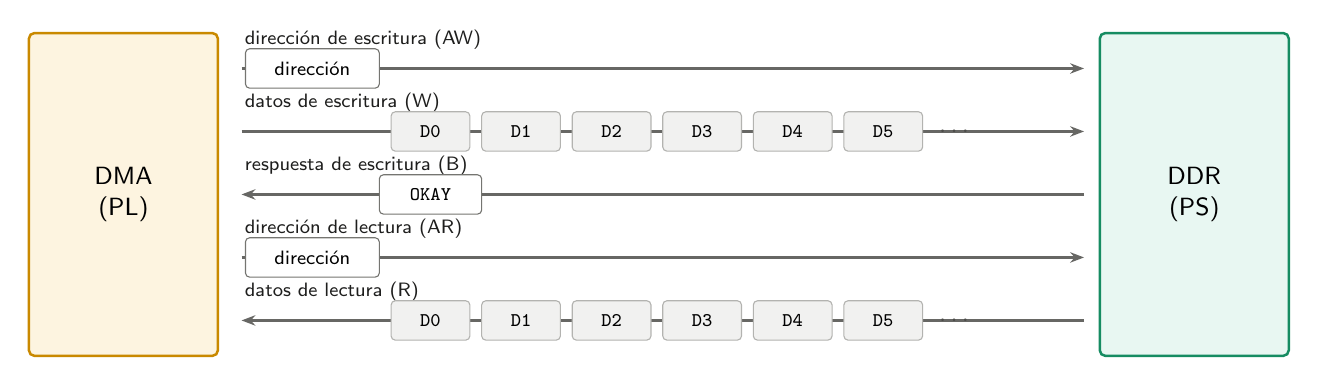
\begin{tikzpicture}[x=1cm, y=1cm, font=\sffamily\small]

\node[ip,  minimum width=2.4cm, minimum height=4.1cm] at (1.2,2.4)  {DMA\\(PL)};
\node[ext, minimum width=2.4cm, minimum height=4.1cm] at (14.8,2.4) {DDR\\(PS)};

\foreach \yy/\nm/\sx/\ex in {%
    4.0/{direcci\'on de escritura (AW)}/2.7/13.4,
    3.2/{datos de escritura (W)}/2.7/13.4,
    2.4/{respuesta de escritura (B)}/13.4/2.7,
    1.6/{direcci\'on de lectura (AR)}/2.7/13.4,
    0.8/{datos de lectura (R)}/13.4/2.7}{%
    \draw[chan] (\sx,\yy) -- (\ex,\yy);
    \node[chname, anchor=west] at (2.7,\yy+0.36) {\nm};
}

\node[addr] at (3.6,4.0) {direcci\'on};
\node[resp] at (5.1,2.4) {\ttfamily OKAY};
\node[addr] at (3.6,1.6) {direcci\'on};

\foreach \i in {0,1,2,3,4,5}{%
    \node[tok] at ({5.1+\i*1.15},3.2) {D\i};
    \node[tok] at ({5.1+\i*1.15},0.8) {D\i};}
\node[dots] at (11.75,3.2) {$\cdots$};
\node[dots] at (11.75,0.8) {$\cdots$};

\end{tikzpicture}
\end{document}
